%
%RESULTS Rev1: Notebook Rev1_13 - A Median & Average Runtime

%
%RESULTS Rev1: Notebook Rev1_13 - B Errors & Timeout percentage
%
In the previous section we saw that the amount of memory is a critical parameter for benchmark performance. 
In this section we study the effect on the query runtimes of increasing the amount of memory to 64GB.
The two leftmost panels of Figure~\ref{fig:Fig02_WatdivVerticalScaling} study the effect of vertical scaling. 
%median / mean
%Bla_N1_32_W1000_Def     8.858862	56.437824
%Gra_N1_32_W1000_Def    47.932701	74.927924
%Es_N1_32_W1000_Def     64.217677	121.887237
%Vir_N1_32_W1000_Def     0.258209	5.622635
%
%Bla_N1_64_W1000_Def     2.825023	6.741764
%Gra_N1_64_W1000_Def    40.375218	59.564284
%Es_N1_64_W1000_Def     35.178332	103.637674
%Vir_N1_64_W1000_Def     0.175917	3.667321
%speedups
%Bla_N1_64_W1000_Def     3	10
%Gra_N1_64_W1000_Def     1  1 
%Es_N1_64_W1000_Def      2  
%Vir_N1_64_W1000_Def     1

\begin{figure*}[htbp!]
	\centering
	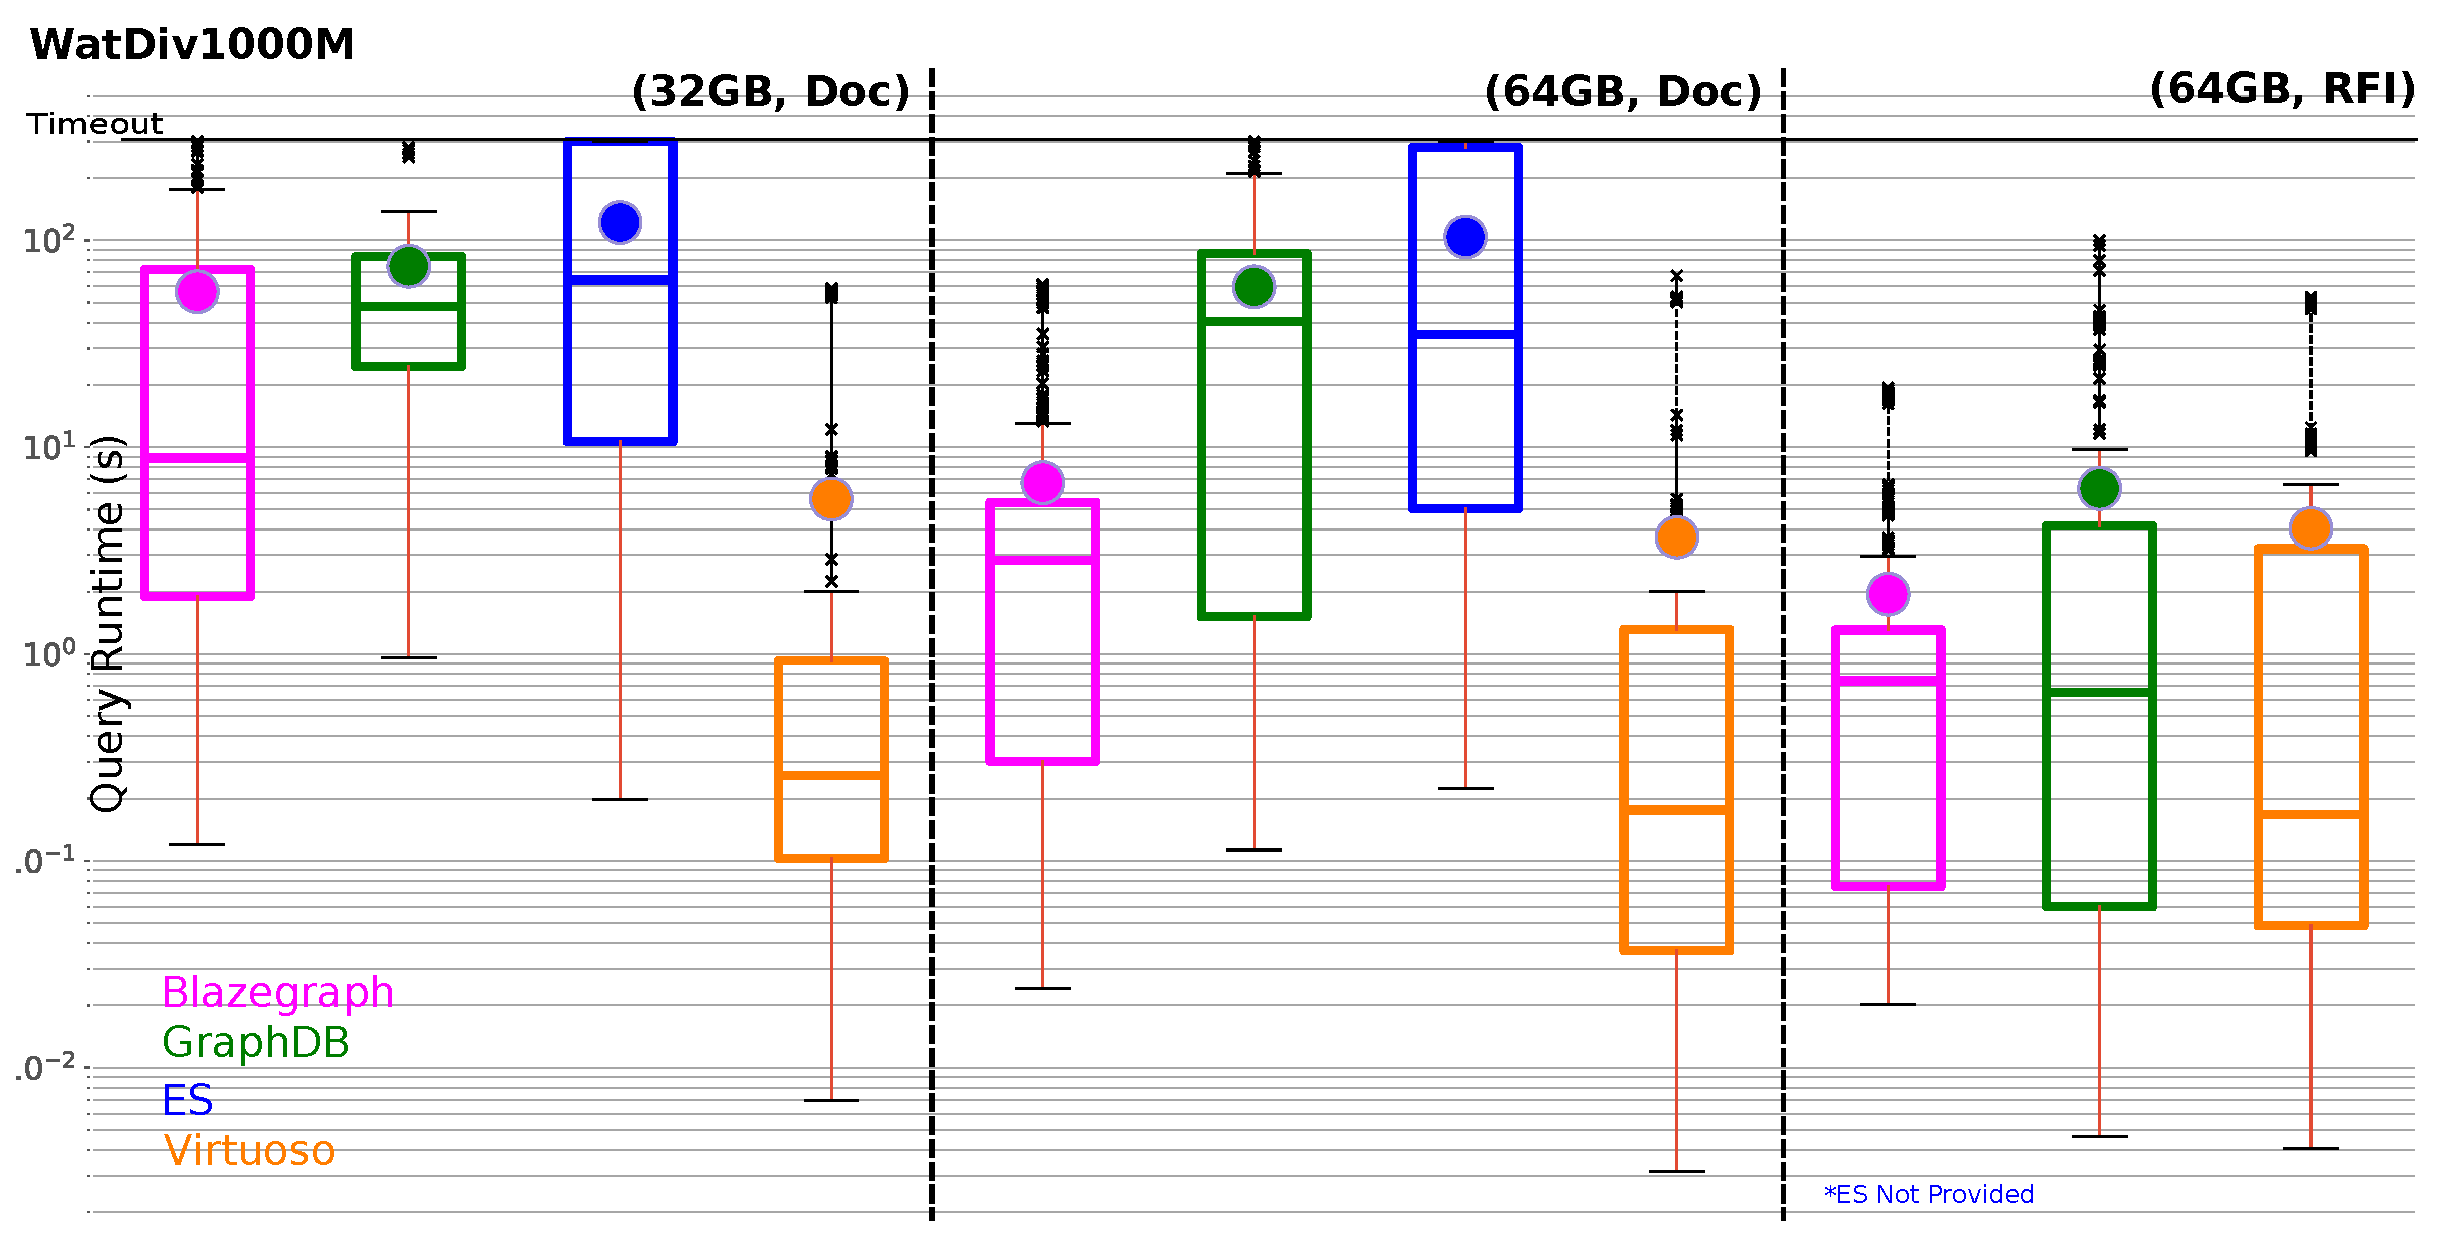
\includegraphics[width=0.9\linewidth]{imgs/Fig02_WatdivVerticalScaling}
	\caption{Query runtime distributions for WatDiv1000M showing the effect of increasing memory from 32GB (left) to 64GB (center) and \emph{Optimized} configurations (right). Virtuoso hardly doesn't benefit from additional memory or better configurations. GraphDB is the most sensitive to proper configuration. In the right panel engine performance starts converging. For batch workloads \textbf{Bla1\_64\_Opt} is the fastest, in terms of median runtimes both \textbf{Vir1\_64\_*} setups perform best.}
	\label{fig:Fig02_WatdivVerticalScaling}
\end{figure*}

\begin{itemize}
	\item \textbf{Memory is no magic solution:} Especially for \textbf{Gra1\_64\_Def} and \textbf{Vir1\_64\_Def} hardly any improvement can be seen. Blazegraph takes full advantage of the additional memory, with a large shift in both median and mean runtimes. The strong hardware dependence of Blazegraph could be a motivation to also study the performance in a GPU setting\footnote{\scriptsize \url{https://www.blazegraph.com/whitepapers/Blazegraph-gpu_InDetail_BloorResearch.pdf}}, which is outside the scope of this work.
	\item \textbf{Speedups:} \textbf{Bla1\_64\_Def} has a speedup of 8.4 for its average runtime and 3.1 for its median runtime. From the other stores only \textbf{ES1\_64\_Def} benefits with a speedup of 1.8 for its average runtime.
	\item \textbf{Benefits for fast queries:} The most outspoken positive effect is the lowering of the lower boundary of the box plots.  
\end{itemize}




%FIGURES ORIGAL PAPER
%FIG_BenchmarkSurvival
%\begin{figure}[ht!]
%	\centering
%	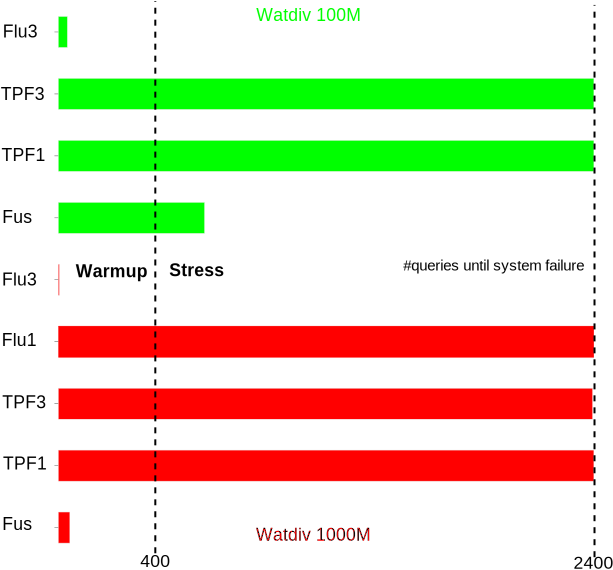
\includegraphics[width=0.99\linewidth]{imgs/F2_BenchmarkSurvival_Other_Reworked}
%	\caption{Benchmark survival for other systems. \textbf{TPF} stays operational for both WatDiv1000M and WatDiv100M. Both as an approach to handle compressed data (\textbf{TPF1})
%		as an approach to support query federation (\textbf{TPF3}) it fulfills its promise of high availability. As of the other approaches only \textbf{Fus} gets passed the warmup phase for WatDiv100M.}
%	\label{fig:F2_BenchmarkSurvival_Other_Reworked}
%\end{figure}
%FIG_ScalingNoSQL
%\begin{figure*}[!ht]
%	\centering
%	\includegraphics[width=0.99\linewidth]{imgs/F6_Scaling_NoSQL_WatDiv1000M_Reworked.eps}
%	\caption{Four panels showing the effect of adding more RAM and \emph{optimized} configurations on the query runtime distribution for WatDiv1000M. In the \emph{optimized} setting Blazegraph and GraphDB share second place. Virtuoso outperforms the other stores even in the 32GB, \emph{default} setup. Adding more memory doesn't impact its performance implying that it doesn't require extra resources. For GraphDB the effect of proper configuration is the most extreme, its performance strongly depends on turning on the correct indexes.}
%	\label{fig:F6_Scaling_NoSQL_WatDiv1000M_Reworked}
%	%\rv{Always name the axes also inside of the figure. I know it's in the caption, but \emph{some} reviewer \emph{will} nag about it.}
%\end{figure*}
